% +==============================================================+
% |  V-modellen                                                  |
% |  Forfatter : aso                                             |
% |  Skole     : AAMS                                            |
% +==============================================================+

\documentclass[12pt, a4paper]{article}

% --- Kodning & sprog ----------------------------------------------------------
\usepackage[utf8]{inputenc}
\usepackage[T1]{fontenc}
\usepackage[danish]{babel}

% --- Layout -------------------------------------------------------------------
\usepackage{geometry}
\geometry{top=2.5cm, bottom=2.5cm, left=3cm, right=3cm, headheight=25pt}

% --- Typografi ----------------------------------------------------------------
\usepackage{lmodern}
\usepackage{microtype}
\usepackage{parskip}

% --- Grafik & farver ----------------------------------------------------------
\usepackage{graphicx}
\usepackage{xcolor}
\usepackage{tikz}
\usetikzlibrary{calc}

% --- Bokse --------------------------------------------------------------------
\usepackage[most]{tcolorbox}

% --- Hyperlinks ---------------------------------------------------------------
\usepackage{hyperref}
\hypersetup{
  colorlinks = true,
  linkcolor  = primaryblue,
  urlcolor   = accentblue,
}

% --- Header & footer ----------------------------------------------------------
\usepackage{fancyhdr}
\usepackage{titlesec}
\usepackage{booktabs}
\usepackage{enumitem}
\usepackage{fontawesome5}

% ==============================================================================
%  FARVEDEFINITIONER
% ==============================================================================
\definecolor{primaryblue}{HTML}{1A3A5C}
\definecolor{accentblue}{HTML}{2E86C1}
\definecolor{lightblue}{HTML}{D6EAF8}
\definecolor{darkgray}{HTML}{555555}
\definecolor{lightgray}{HTML}{F4F6F7}
\definecolor{successgreen}{HTML}{1E8449}
\definecolor{lightgreen}{HTML}{D5F5E3}
\definecolor{warnorange}{HTML}{E67E22}
\definecolor{lightyellow}{HTML}{FEF9E7}
\definecolor{siemensblue}{HTML}{009999}

% ==============================================================================
%  TCOLORBOX STILE
% ==============================================================================
\tcbset{
  infobox/.style={
    enhanced,
    colback   = lightblue,
    colframe  = accentblue,
    coltitle  = white,
    fonttitle = \bfseries,
    arc       = 3pt,
    boxrule   = 1pt,
    title style={fill=accentblue},
  },
  tipbox/.style={
    enhanced,
    colback   = lightgreen,
    colframe  = successgreen,
    coltitle  = white,
    fonttitle = \bfseries,
    arc       = 3pt,
    boxrule   = 1pt,
    title style={fill=successgreen},
  },
  warnbox/.style={
    enhanced,
    colback   = lightyellow,
    colframe  = warnorange,
    coltitle  = white,
    fonttitle = \bfseries,
    arc       = 3pt,
    boxrule   = 1pt,
    title style={fill=warnorange},
  },
  defbox/.style={
    enhanced,
    colback   = lightgray,
    colframe  = primaryblue,
    coltitle  = white,
    fonttitle = \bfseries,
    arc       = 3pt,
    boxrule   = 1pt,
    title style={fill=primaryblue},
  },
}

% ==============================================================================
%  HEADER & FOOTER
% ==============================================================================
\pagestyle{fancy}
\fancyhf{}
\fancyhead[L]{\textcolor{darkgray}{\small\textit{V-modellen}}}
\fancyhead[R]{\textcolor{darkgray}{\small\textit{AAMS | aso}}}
\fancyhead[C]{\textcolor{siemensblue}{\rule[-2pt]{0pt}{12pt}\small\faIndustry}}
\renewcommand{\headrulewidth}{1pt}
\fancyfoot[C]{\textcolor{darkgray}{\small\thepage}}
\fancyfoot[R]{\textcolor{darkgray}{\small\today}}

% ==============================================================================
%  SEKTIONSFORMATERING
% ==============================================================================
\titleformat{\section}
  {\color{primaryblue}\Large\bfseries}
  {\color{siemensblue}\thesection\hspace{6pt}\textcolor{siemensblue}{|}\hspace{6pt}}
  {0pt}{}[{\color{siemensblue}\titlerule[1pt]}]

\titleformat{\subsection}
  {\color{primaryblue}\large\bfseries}
  {\color{accentblue}\thesubsection\hspace{6pt}}
  {0pt}{}

\titlespacing{\section}{0pt}{18pt}{8pt}
\titlespacing{\subsection}{0pt}{12pt}{4pt}

% ==============================================================================
%  DOKUMENT START
% ==============================================================================
\begin{document}

% -----------------------------------------------------------------------------
%  FORSIDE
% -----------------------------------------------------------------------------
\begin{titlepage}
\thispagestyle{empty}

\begin{tikzpicture}[remember picture, overlay]
  % Øverste farvede banner
  \fill[primaryblue]
    (current page.north west) rectangle
    ([yshift=-4.5cm] current page.north east);

  % Teal dekorativt bånd
  \fill[siemensblue]
    ([yshift=-4.5cm] current page.north west) rectangle
    ([yshift=-5.0cm] current page.north east);

  % Tyndt accentstribe
  \fill[accentblue]
    ([yshift=-5.0cm] current page.north west) rectangle
    ([yshift=-5.15cm] current page.north east);

  % Dekorativt ikon – højre side
  \node[anchor=east, xshift=-1.5cm, yshift=-2.3cm]
    at (current page.north east)
    {\textcolor{white!20!primaryblue}{\fontsize{90}{90}\selectfont\faIndustry}};

  % Skole-tekst
  \node[anchor=north west, xshift=2cm, yshift=-0.7cm]
    at (current page.north west)
    {\textcolor{white!70!primaryblue}\large\bfseries AAMS --- Automationsteknolog};

  % Fag-tekst
  \node[anchor=north west, xshift=2cm, yshift=-1.3cm]
    at (current page.north west)
    {\textcolor{white!60!primaryblue}\normalsize Teknologi og Projektudvikling $\cdot$ 2.\ Semester};

  % Hoved-titel
  \node[anchor=north west, xshift=2cm, yshift=-2.2cm]
    at (current page.north west)
    {\textcolor{white}{\fontsize{24}{30}\selectfont\bfseries V-modellen}};

  % Undertitel
  \node[anchor=north west, xshift=2.1cm, yshift=-3.7cm]
    at (current page.north west)
    {\textcolor{white!80!siemensblue}\large\itshape Udvikling og test af automationssystemer};

  % Bundlinje
  \fill[lightgray]
    ([yshift=3.5cm] current page.south west) rectangle
    ([yshift=2.0cm] current page.south east);
  \fill[accentblue]
    ([yshift=3.5cm] current page.south west) rectangle
    ([yshift=3.35cm] current page.south east);

  \node[anchor=west, xshift=2cm, yshift=2.8cm]
    at (current page.south west)
    {\textcolor{primaryblue}{\faUserCircle\quad\textbf{Forfatter:} aso
     \quad\textcolor{darkgray}{|}\quad
     \faCalendar\quad\textbf{Dato:} \today
     \quad\textcolor{darkgray}{|}\quad
     \faUniversity\quad\textbf{Skole:} AAMS}};
\end{tikzpicture}

\vspace*{5.5cm}

\begin{center}
\begin{tcolorbox}[
  enhanced,
  width=13cm,
  colback=lightgray,
  colframe=primaryblue,
  arc=5pt,
  boxrule=1.5pt,
  title={\faInfoCircle\quad Læringsmål},
  coltitle=white,
  fonttitle=\bfseries,
  title style={fill=primaryblue},
]
\begin{itemize}[leftmargin=1.2em, itemsep=4pt]
  \item[\textcolor{siemensblue}{\faCheckCircle}]
    Kende V-modellens struktur og de ni trin
  \item[\textcolor{siemensblue}{\faCheckCircle}]
    Forstå forskellen på \textit{Verification} og \textit{Validation}
  \item[\textcolor{siemensblue}{\faCheckCircle}]
    Kende koblinger mellem designtrin og testtrin
  \item[\textcolor{siemensblue}{\faCheckCircle}]
    Kunne applicere modellen på et konkret automationsprojekt
  \item[\textcolor{siemensblue}{\faCheckCircle}]
    Vide hvornår FAT, SAT og UAT hører hjemme i modellen
\end{itemize}
\end{tcolorbox}
\end{center}

\end{titlepage}

% -----------------------------------------------------------------------------
%  INDHOLDSFORTEGNELSE
% -----------------------------------------------------------------------------
\newpage
\thispagestyle{fancy}
\tableofcontents
\newpage

% ==============================================================================
\section{Introduktion}
% ==============================================================================

V-modellen er en måde at strukturere udvikling og test af et automationssystem.
Venstre side handler om at \textbf{definere og designe}, bunden er selve \textbf{implementeringen}, og højre side er \textbf{test og verifikation}.

Pointen er, at hvert trin på venstre side har et modsvarende testtrin på højre side. Det er ikke tilfældigt --- det er meningen.

\begin{tcolorbox}[defbox, title={\faBook\quad To centrale begreber}]
\begin{itemize}[leftmargin=1.2em, itemsep=4pt]
  \item[\textcolor{accentblue}{\faBolt}]
    \textbf{Verification} --- bygger vi systemet rigtigt (følger vi designet)?
  \item[\textcolor{accentblue}{\faBolt}]
    \textbf{Validation} --- bygger vi det rigtige system (løser det opgaven)?
\end{itemize}
\vspace{4pt}
Det er ikke det samme, og begge dele er vigtige.
\end{tcolorbox}

\vspace{0.5cm}
\begin{center}
  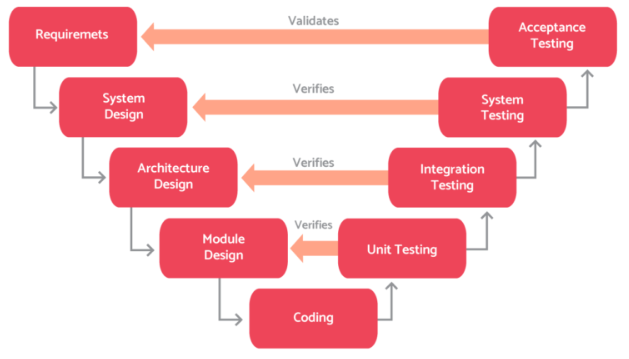
\includegraphics[width=0.92\textwidth]{v-modellen.png}
\end{center}

% ==============================================================================
\section{Venstre side --- design og specifikation}
% ==============================================================================

% ------------------------------------------------------------------------------
\subsection{Requirements --- kravspecifikation}
% ------------------------------------------------------------------------------

Det første trin handler om at beskrive, hvad systemet skal kunne. Ikke \textit{hvordan} --- det kommer senere --- men \textit{hvad}.

Det er her man samler krav fra kunden, brugeren eller processen. I praksis spænder det fra ret overordnede ting til mere konkrete krav om svartider, sikkerhedsfunktioner og kommunikation.

\begin{tcolorbox}[infobox, title={\faListUl\quad Eksempler på krav}]
\begin{itemize}[leftmargin=1.2em, itemsep=2pt]
  \item Anlægget skal starte og stoppe fra HMI
  \item En motor må ikke starte, hvis en sikkerhedsbetingelse ikke er opfyldt
  \item Data skal kunne trækkes fra PLC til PC
  \item Kommunikationsforsinkelse må ikke overstige \textit{X} ms
  \item Anlægget skal give alarmer og kunne håndtere fejl
\end{itemize}
\end{tcolorbox}

Man skelner gerne mellem: funktionskrav, sikkerhedskrav, driftskrav, kommunikationskrav og krav til brugerbetjening.

Det man skal have ud af fasen er en kravspecifikation --- det hedder nogle gange en \textbf{URS} (User Requirements Specification).
Det er det dokument, man til sidst tester imod i accepttesten.

% ------------------------------------------------------------------------------
\subsection{System Design --- systemdesign}
% ------------------------------------------------------------------------------

Nu omsætter man kravene til en samlet teknisk løsning, men stadig på et overordnet niveau.
Man beslutter hvilke hoveddele systemet består af og groft hvordan de spiller sammen --- PLC, HMI, sensorer, netværk, eventuel PC eller database osv.

Man laver \textit{ikke} kode her. Det handler om systemets struktur.

Det er her man typisk laver blokdiagrammer, netværksoversigter og beslutter, hvad der skal ligge i hvad.
Fx: PLC styrer processen, HMI bruges til lokal betjening, og en Python-applikation trækker data til logging via Snap7.

\begin{tcolorbox}[tipbox, title={\faCheckSquare\quad Output fra fasen}]
Systembeskrivelse, blokdiagram, hardwareoversigt, overordnet funktionsfordeling.
\end{tcolorbox}

% ------------------------------------------------------------------------------
\subsection{Architecture Design --- arkitekturdesign}
% ------------------------------------------------------------------------------

Her går man et niveau ned og definerer, hvordan systemets dele konkret hænger sammen.
Det handler ikke bare om ``PLC snakker med HMI'' --- man skal beskrive hvad der overføres, via hvilke interfaces og i hvilken retning.

Man fastlægger bl.a.:

\begin{itemize}[leftmargin=1.5em, itemsep=2pt]
  \item Ansvarsfordeling --- hvad styres og besluttes hvor
  \item Interfaces og dataflow
  \item Kommunikationsstruktur
  \item Navngivning og struktur i software og data
\end{itemize}

I et Snap7-projekt er det fx her man beslutter IP-adresser, hvilke DB'er der eksponeres, og hvilke adresser og datatyper der bruges.
Det er altså mere end bare ``IP-konfiguration'' --- det er selve den tekniske struktur for samspillet.

\begin{tcolorbox}[tipbox, title={\faCheckSquare\quad Output fra fasen}]
Interfacebeskrivelser, dataflow, softwarearkitektur, adresse- og tagstruktur.
\end{tcolorbox}

% ------------------------------------------------------------------------------
\subsection{Module Design --- moduldesign}
% ------------------------------------------------------------------------------

Her beskrives de enkelte funktioner i detaljer.
Et modul kan fx være motorstyring, en ventilsekvens, temperaturregulering eller alarmhåndtering --- én afgrænset funktion.

Det er på dette niveau, man designer den konkrete styringslogik:

\begin{itemize}[leftmargin=1.5em, itemsep=2pt]
  \item Sekvensforløb og state machine
  \item Interlocks og permissives
  \item Alarmer, resetlogik
  \item Manuelle og automatiske funktioner
  \item Funktionsblokke og parametre
\end{itemize}

Et motormodul kan fx have tilstandene:

\begin{center}
\begin{tcolorbox}[
  enhanced,
  colback=lightgray,
  colframe=primaryblue,
  arc=3pt,
  boxrule=0.8pt,
  width=10cm,
]
\centering\ttfamily
Stopped \textrightarrow{} Starting \textrightarrow{} Running \textrightarrow{} Fault \textrightarrow{} Reset
\end{tcolorbox}
\end{center}

Man beslutter præcist hvilke betingelser der skal være opfyldt for at motoren må starte, og hvad der stopper den igen.

\begin{tcolorbox}[tipbox, title={\faCheckSquare\quad Output fra fasen}]
Funktionsbeskrivelser, sekvensdiagrammer, state machines, FB-design.
\end{tcolorbox}

% ------------------------------------------------------------------------------
\subsection{Coding --- implementering}
% ------------------------------------------------------------------------------

Nu laves selve programmet og den fysiske løsning.
Det kan være PLC-kode, HMI-billeder, alarmopsætning, netværkskonfiguration eller Python-kode til Snap7.

\begin{tcolorbox}[warnbox, title={\faExclamationTriangle\quad Vigtigt}]
Kodningen skal \textbf{følge designet}. Man bør ikke ``finde på løsninger undervejs'' --- det giver dårlig sporbarhed og gør det sværere at teste bagefter.
\end{tcolorbox}

\begin{tcolorbox}[tipbox, title={\faCheckSquare\quad Output fra fasen}]
Færdigt PLC-program, HMI-projekt, kommunikationsopsætning, kode.
\end{tcolorbox}

% ==============================================================================
\section{Højre side --- test og verifikation}
% ==============================================================================

Nu testes systemet trin for trin mod det der blev designet på venstre side.

% ------------------------------------------------------------------------------
\subsection{Unit Testing --- modultest}
% ------------------------------------------------------------------------------

Her testes de enkelte moduler isoleret. Altså én funktion ad gangen:

\begin{itemize}[leftmargin=1.5em, itemsep=2pt]
  \item Virker motorblokken rigtigt?
  \item Skifter state machine korrekt mellem Idle, Run og Fault?
  \item Reagerer alarmmodulet som forventet?
\end{itemize}

I PLC-sammenhæng bruger man her simulation, forcing af signaler og kontrol af transitions.
Formålet er at sikre at hver funktion virker, inden man kobler den sammen med resten.

% ------------------------------------------------------------------------------
\subsection{Integration Testing --- integrationstest}
% ------------------------------------------------------------------------------

Her testes om modulerne virker korrekt \textbf{sammen}.
Man tester nu de interfaces og sammenhænge man definerede i Architecture Design.

\begin{tcolorbox}[infobox, title={\faListUl\quad Eksempler}]
\begin{itemize}[leftmargin=1.2em, itemsep=2pt]
  \item PLC og HMI udveksler de rigtige data
  \item Python med Snap7 kan læse og skrive korrekte værdier i PLC
  \item Alarmer vises rigtigt på HMI
  \item Frekvensomformer reagerer korrekt på PLC-kommandoer
\end{itemize}
\end{tcolorbox}

Formålet er at sikre at grænseflader og kommunikation fungerer i praksis.

% ------------------------------------------------------------------------------
\subsection{System Testing --- systemtest}
% ------------------------------------------------------------------------------

Her testes hele det samlede system som én enhed --- svarer til System Design-trinnet.

Man kigger nu på om hele løsningen opfører sig som beskrevet: starter anlægget korrekt, virker sekvenser i rækkefølge, fungerer betjening fra HMI, håndteres fejl og reset som planlagt?

\begin{tcolorbox}[infobox, title={\faInfoCircle\quad FAT og systemtest}]
I automationsprojekter ligner dette typisk en \textbf{FAT} (Factory Acceptance Test), men det er vigtigt at skelne: FAT er en praktisk testform, systemtest er V-modellens faglige testniveau.
\end{tcolorbox}

% ------------------------------------------------------------------------------
\subsection{Acceptance Testing --- accepttest}
% ------------------------------------------------------------------------------

Her vurderes om systemet opfylder de \textbf{oprindelige krav} og kan godkendes.
Accepttesten modsvarer Requirements-fasen.

Man validerer nu om systemet løser den opgave det blev bestilt til: er kravene opfyldt, kan operatøren bruge systemet, er kapacitet og svartider i orden?

I praksis hedder det \textbf{SAT} (Site Acceptance Test) eller \textbf{UAT} (User Acceptance Test), afhængigt af projektet.

% ==============================================================================
\section{Koblinger i modellen}
% ==============================================================================

Det centrale i V-modellen er de direkte koblinger mellem venstre og højre side:

\vspace{0.4cm}
\begin{center}
\begin{tcolorbox}[
  enhanced,
  colback=lightgray,
  colframe=primaryblue,
  arc=4pt,
  boxrule=1pt,
  width=11cm,
]
\begin{tabular}{r@{\quad\textcolor{accentblue}{$\leftrightarrow$}\quad}l}
  \textbf{Requirements}      & \textbf{Acceptance Testing} \\[4pt]
  \textbf{System Design}     & \textbf{System Testing}     \\[4pt]
  \textbf{Architecture Design} & \textbf{Integration Testing} \\[4pt]
  \textbf{Module Design}     & \textbf{Unit Testing}       \\
\end{tabular}
\end{tcolorbox}
\end{center}
\vspace{0.4cm}

Hvert designtrin skal altså kunne testes.
Hvis man ikke kan formulere en test for et designtrin, er designet sandsynligvis ikke præcist nok.

% ==============================================================================
\section{Et konkret eksempel}
% ==============================================================================

\begin{tcolorbox}[infobox, title={\faInfoCircle\quad Opgaven}]
Operatøren skal kunne starte og stoppe en motor fra HMI, og en PC skal kunne læse motorstatus via Snap7.
\end{tcolorbox}

\vspace{0.3cm}

\begin{center}
\begin{tabular}{lp{9.5cm}}
\toprule
\textbf{Trin} & \textbf{Indhold} \\
\midrule
Krav          & Start/stop fra HMI, læs motorstatus fra PC via Snap7 \\[4pt]
Systemdesign  & PLC, HMI, motorstarter og PC med Python \\[4pt]
Arkitekturdesign & PLC styrer og håndterer sikkerhedslogik. HMI sender kommandoer og viser status. Python læser DB via Snap7 \\[4pt]
Moduldesign   & Motormodul: start, stop, fejl, reset, statusbits, interlock mod overlast \\[4pt]
Kodning       & PLC-program, HMI-billede og Python-script \\[4pt]
Modultest     & Test af motormodulet alene \\[4pt]
Integrationstest & PLC–HMI og PLC–PC kommunikation \\[4pt]
Systemtest    & Hele motorstyringen som samlet funktion \\[4pt]
Accepttest    & Kan operatøren bruge løsningen, og er kravene opfyldt? \\
\bottomrule
\end{tabular}
\end{center}

% ==============================================================================
\section{Opsummering}
% ==============================================================================

V-modellen er en udviklings- og testmodel, hvor krav og design specificeres på venstre side, implementeres i bunden og verificeres/valideres på højre side.

\begin{tcolorbox}[tipbox, title={\faCheckCircle\quad Hvorfor bruge V-modellen?}]
\begin{itemize}[leftmargin=1.2em, itemsep=4pt]
  \item[\textcolor{successgreen}{\faArrowRight}]
    Tydelig sammenhæng mellem krav, design, programmering og test
  \item[\textcolor{successgreen}{\faArrowRight}]
    Lettere at arbejde systematisk og dokumentere hvad der er gjort
  \item[\textcolor{successgreen}{\faArrowRight}]
    Tidlige fejl opdages --- ikke kun til sidst ved accepttest
  \item[\textcolor{successgreen}{\faArrowRight}]
    Bruges bredt i industrien under navne som FAT, SAT og UAT
\end{itemize}
\end{tcolorbox}

\end{document}
